\documentclass{article}

\usepackage{tikz}

\begin{document}

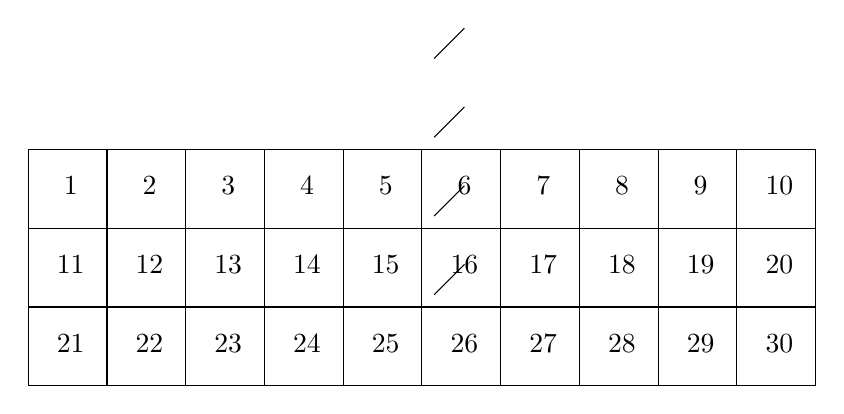
\begin{tikzpicture}
%\foreach \x in{0,...,4}
%{   \draw (0,\x ,4) -- (4,\x ,4); %horizontal front
%	\draw (\x ,0,4) -- (\x ,4,4); %vertical front
%	
%	\draw (4,\x ,4) -- (4,\x ,0);%horizontal top
%	\draw (\x ,4,4) -- (\x ,4,0);%vertical top
%	
%	\draw (4,0,\x ) -- (4,4,\x ); 
%	\draw (0,4,\x ) -- (4,4,\x );
%}

\foreach \x in{1,...,4}
{ 	\draw (0,\x ,4) -- (10,\x ,4); %horizontal front }
}
	
\foreach \x in{0,...,10}	
{	\draw (\x ,1,4) -- (\x ,4,4); %vertical front }
}

\foreach \x in{1,...,4}
{	\draw (4,\x ,) -- (4,\x ,0);%horizontal top
}
%	\draw (\x ,4,4) -- (\x ,4,0);%vertical top
	
%	\draw (4,0,\x ) -- (4,4,\x ); 
%	\draw (0,4,\x ) -- (4,4,\x );




\foreach \x in{1,...,10}{    
    \foreach \y in{0,...,2}{
        \node[] at (\x-2,2-\y) {\pgfmathprint{int(\x+10*\y)}};
    }
}
\end{tikzpicture}

\end{document}
